\documentclass{article}

\usepackage[margin=1.25in]{geometry}
\usepackage{graphicx}
\usepackage{subcaption}
\usepackage{amsmath}
\usepackage[svgnames]{xcolor}
\usepackage[colorlinks=true, linkcolor=Maroon, urlcolor=Blue]{hyperref}
\usepackage{svg}

\begin{document}
    \title{Reproducing results from the Urban Traffic Control paper}
    \author{Jakub Filipek (balbok)}
    \maketitle

    \section{Introduction}
    \label{sec:intro}
    The Urban Traffic Control paper~\cite{utc} is interesting because it combines Reinforcement Learning with more-complex cases of Urban Traffic Control (UTC).
    UTC is hard because state spaces are vast and relations between traffic lights are not well understood.
    Furthermore, there has not yet been a good example of RL approach solving systems of intersections with complexity similar to large city centers.

    While~\cite{utc} doesn't necessarily solve the second issue, the proposed method scales well with number of intersections,
    which may generalize to much more complex systems than 3-by-3 grid explored in original paper, and this reproduction attempt.

    \section{Environment}
    \subsection{State Space}
    \begin{figure}[h]
        \centering
        \begin{subfigure}[b]{0.6\linewidth}
            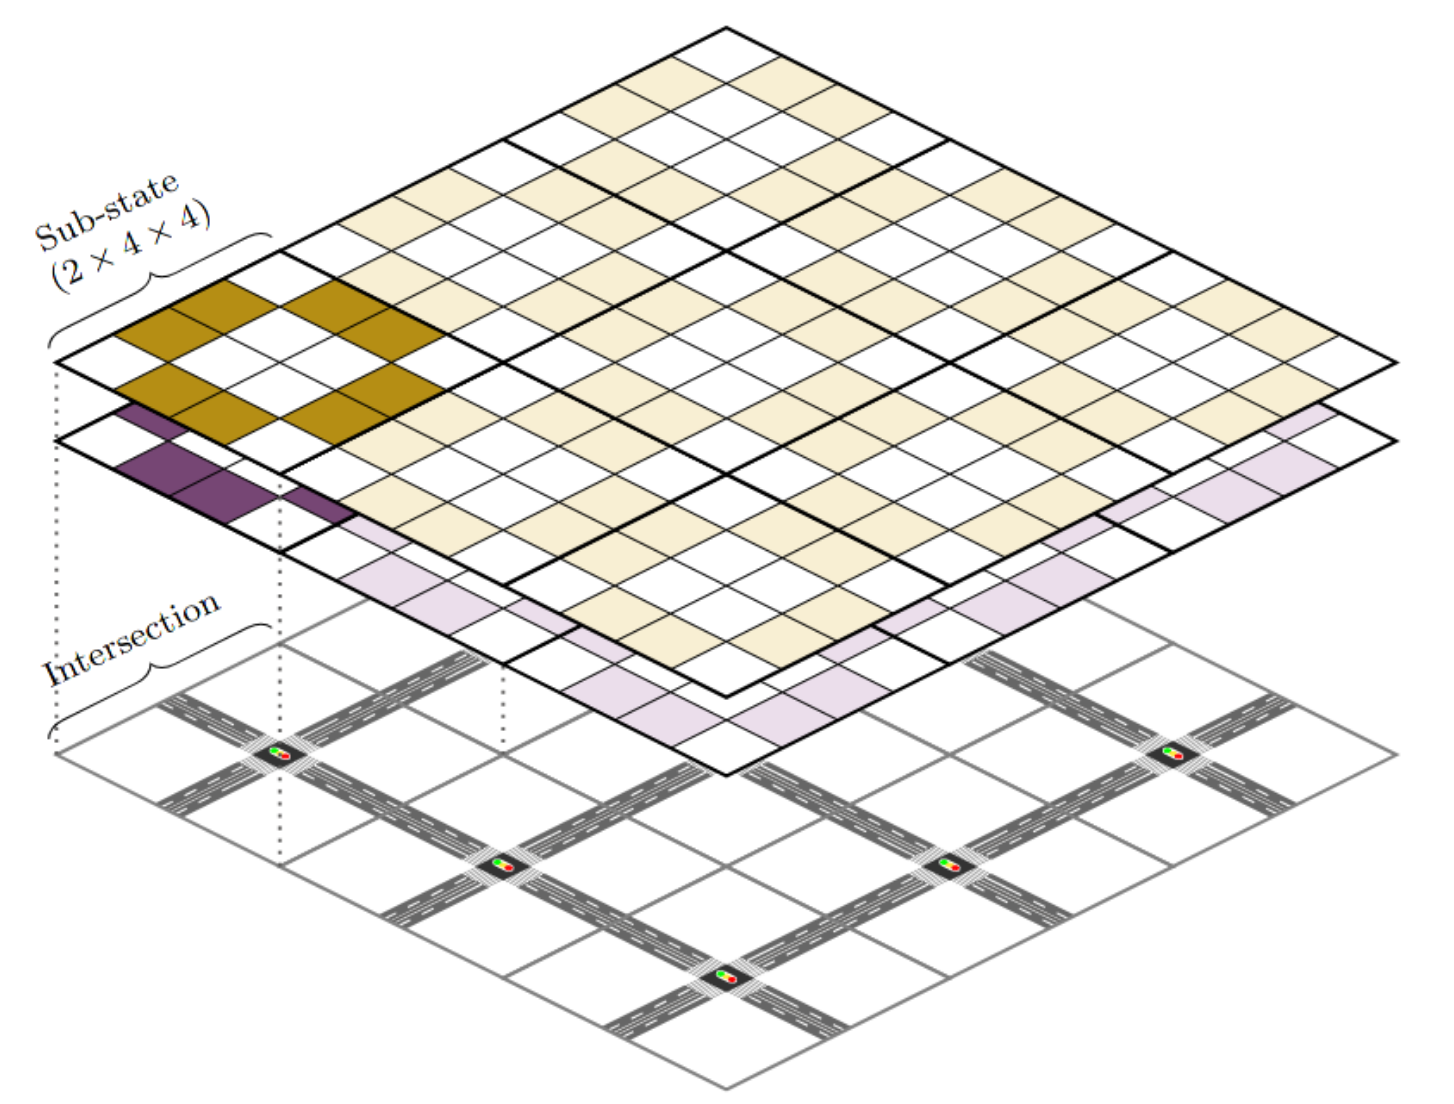
\includegraphics[width=\linewidth]{figs/state-space.png}
            \caption{Network to state space conversion.}
        \end{subfigure}
        \begin{subfigure}[b]{0.3\linewidth}
            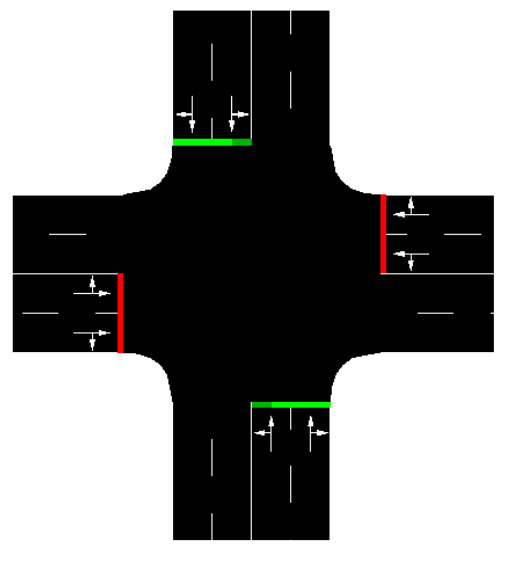
\includegraphics[width=\linewidth]{figs/intersection.png}
            \caption{Intersection visualization in SUMO.}
        \end{subfigure}
        \caption{
            State space representation.
            On the left, each traffic light is converted into a $2x4x4$ tensor, were detector from each incoming lane contributes two features.
            The right shows a SUMO representation of a single intersection for reference.
        }
        \label{fig:state-space}
    \end{figure}

    The state space is $R^{2\times12\times12}$.
    It consists of 9 ($3\times3$) $R^{2\times4\times4}$ segments, each representing a traffic light.
    For each traffic light there are 150m detectors (not visualized) on each of the incoming lanes (500m each).
    For each lane two features are captured (mean speed of vehicles on the detector, number of halted vehicles).
    Hence there is sixteen features for each intersection.
    They are aranged into a $2\times4\times4$ space, with first dimension for the two features,
    and $4\times4$ grid capturing the orientation of each incoming lane (North, West etc.).

    Fig.~\ref{fig:state-space} shows visualization of the state space, as presented in~\cite{utc}.

    \subsubsection{Additional state features}
    \label{sec-sub:add-feats}
    One perhaps missing part in state representation is the state of traffic lights themselves.
    In original work, the agent has no information whether which phase (See Fig.~\ref{fig:phases}) the traffic lights are currently on.

    To address this concern I added additional feature for traffic light state.
    As every incoming lane has two outlet lanes (left/straight or straight/right), this feature is defined as a sum:
    \begin{align*}
        f(i) = \sum\limits_{o \in OUT(i)} \begin{cases}
            0.75 & \text{if $o$ is green} \\
            0.25 & \text{if $o$ is yellow} \\
            0.0 & \text{if $o$ is red} \\
        \end{cases}
    \end{align*}
    where $i$ is incoming lane and $o$ is a state of traffic light between $i$ and some outlet lane (given by relation $OUT$).

    Hence in this case the resulting state space is $R^{3\times12\times12}$.

    \subsection{Action Space}
    The Action Space is $\{0, 1\}^9$. For each traffic light the phase can be changed (1) or remain the same (0).

    \begin{figure}[h]
        \centering
        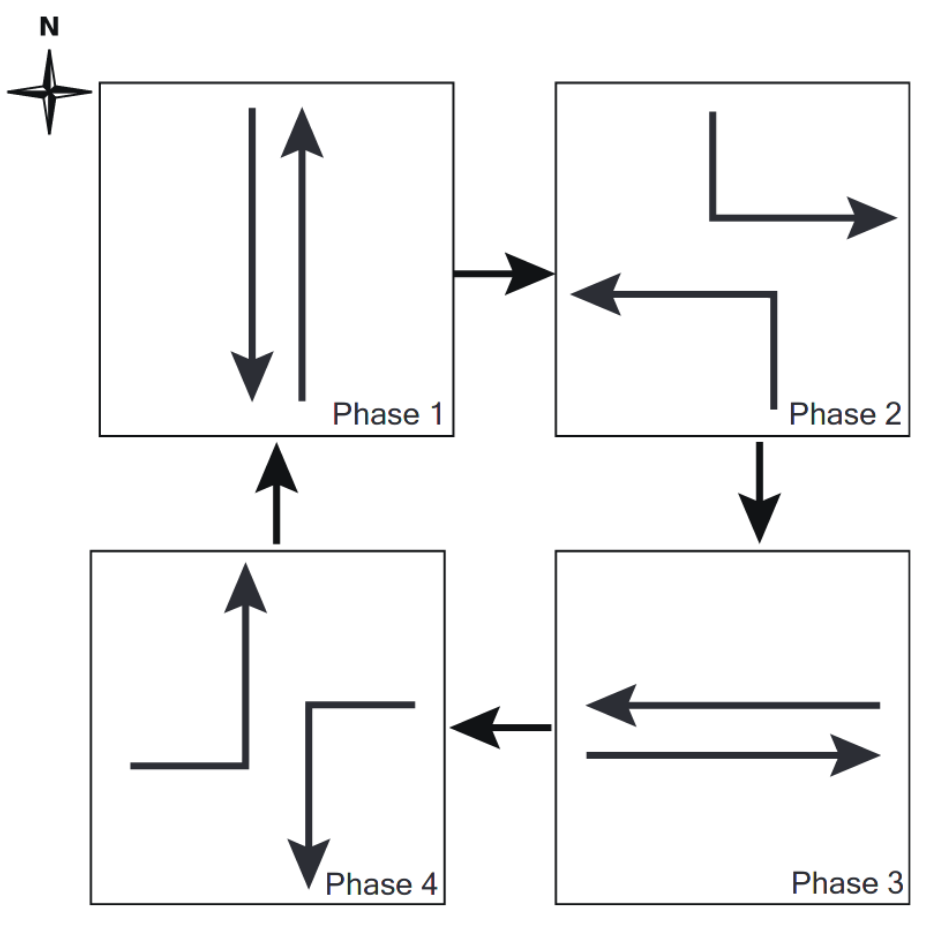
\includegraphics[width=0.4\linewidth]{figs/phases.png}
        \caption{
            4 phases of a traffic light.
            The light oscillate between straight and left turn, and NS/WE directions.
            Right turn is always on, as it does not collide with any other movements.
            There are also yellow light phases corresponding to each of the arrows on the figure.
        }
        \label{fig:phases}
    \end{figure}

    There are two caveats however. First is that traffic light cannot be changed if it has any yellow lights.
    This is done mostly due to the simulation, where cars can perform instant breaking with no reaction time, thus making it unrealistic.
    Setting yellow light phases time to 3 seconds makes this reproduction attempt avoid this problem and be consistent with~\cite{utc}.

    Secondly, lights can change on its own, which is an artifact of SUMO.
    This is most important in case of yellow lights, as automatic iteration is the only way phase can change in that case.
    In all other cases agent can invoke change of light (with 1), but if enough time has passed SUMO will change a light due to cycling of a light.
    To avoid this problem I set phase duration for non-yellow light phases to 600 seconds.
    Without agent (action is always $0^9$) network becomes clogged.
    Such behavior is crucial for agent to not depend on pre-set cycles, but it is not at all described in~\cite{utc} and might lead to differences in the results.

    \subsection{Reward function}
    The reward function involves both global part, which purpose is to evaluate throughput of the network,
    and local part, which balances intersections.

    The global reward function is:
    \begin{align}
        R_g = |V_{out}| - |V_{in}| \\
        \label{eq:reward-global}
    \end{align}
    where $V_{out}$ and $V_{in}$ are numbers of outgoing and incoming vehicles, respectively.
    The vehicles which teleported out of the network are not included, making calculation consistent with original work.

    The local reward function is:
    \begin{align}
        R_l(i) = -|\max q_i^\text{WE} - \max q_i^\text{NS}| \\
        \label{eq:reward-local}
    \end{align}
    for each intersection $i$. $q_i^\text{WE}$ denotes lengths of queues for east- and westbound traffic.
    Similar definition is used for $q_i^\text{NS}$.

    Overall, combining Eqs.~\ref{eq:reward-global} and~\ref{eq:reward-local} we get:
    \begin{align}
        R = \beta R_g + (1 - \beta) \frac{1}{N_{TLS}} \sum\limits_{i}^{N_{TLS}}R_l(i)
    \end{align}
    where $\beta$ changes linearly during training from $0$ to $1$.
    This ensures that agent first solves local problems, then moving to optimization of global network.

    \section{Agent}
    Both the Actor/Critic model and PPO+GAE algorithm has been well described by the original paper in Sections
    \href{https://arxiv.org/pdf/1808.01876.pdf#subsection.3.4}{IIID} and \href{https://arxiv.org/pdf/1808.01876.pdf#subsection.3.5}{IIIE},
    respectively.

    \subsection{ResNet Based CNN}
    \begin{figure}[h]
        \centering
        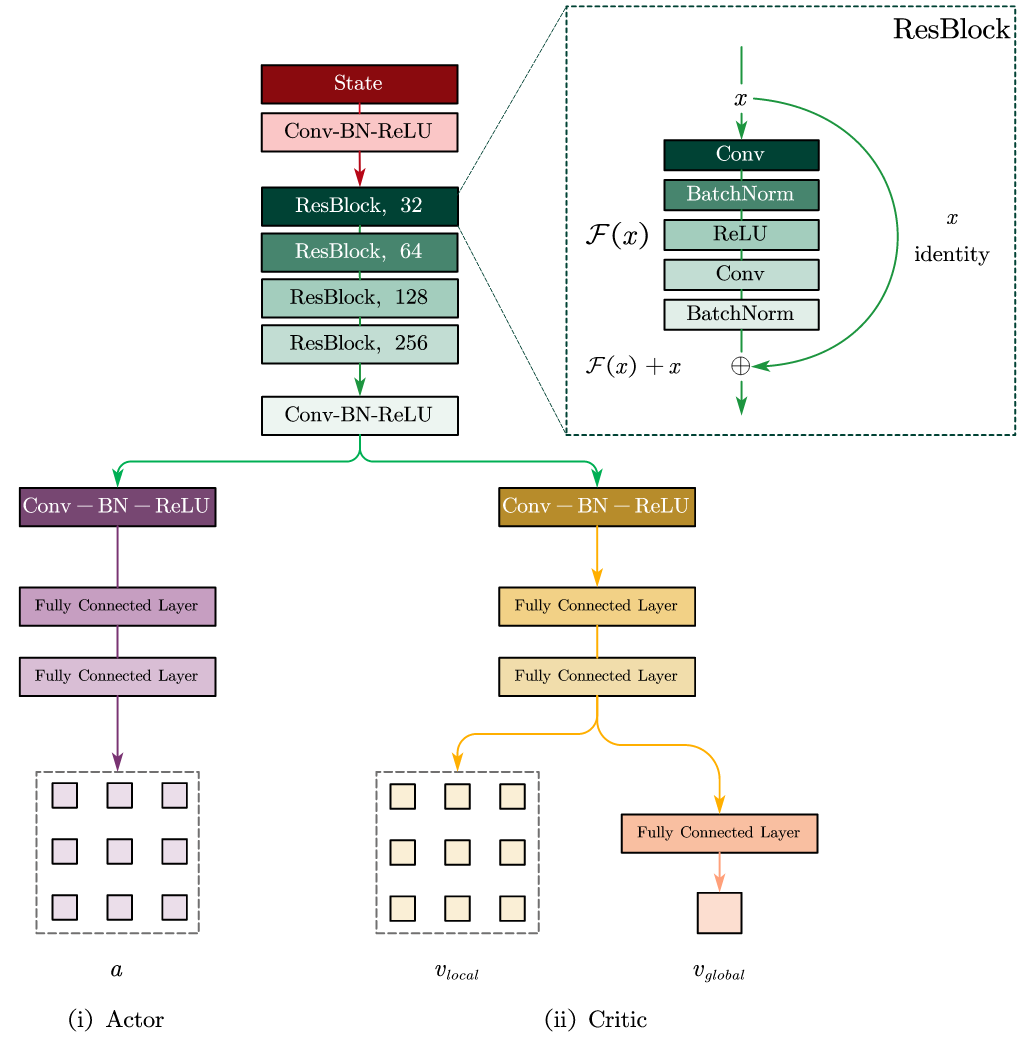
\includegraphics[width=0.4\linewidth]{figs/cnn.png}
        \caption{
            Visualization of the CNN architecture as described in~\cite{utc}.
        }
        \label{fig:cnn}
    \end{figure}

    While~\ref{fig:cnn} describes architecture well, both it and the original text omit some hyper-parameters.
    Size of kernels and channels for Convolutions in non-ResBlocks has been omitted.
    In this case for the first such layer I used a $3\times3$ convolution with 32 channels.
    For remaining convolutions I used a $4\times4$ kernel, motivated by size of single traffic light in state representation,
    along with 32 channels.

    Another unspecified hyperparameter was in size of fully-connected layers, which I set to be $(256, 32), (32, 1 (\text{Critic}) \text{ or } 2 (\text{Actor}))$.

    Lastly, for sake of verbosity, the output shapes corresponding to variables on Fig.~\ref{fig:cnn} are as follows:
    \begin{align*}
        a &\in R^{9\times2} &
        v_{local} &\in R^{9} &
        v_{global} &\in R \\
    \end{align*}

    \subsection{PPO + GAE}
    Proximal Policy Optimization (PPO)~\cite{ppo} has proven to be a widely successful algorithm in variety of problems.
    As the original (UTC) paper claims its monotonic improvement through probability ratios is preferred in case of complex systems
    such as set of traffic lights.

    The description is clear and exact in the original work (\href{https://arxiv.org/pdf/1808.01876.pdf#subsection.3.5}{Section IIIE}),
    I will not repeat the description of common PPO parameters.
    However for reference the parameters are shown in Table~\ref{tab:ppo-hyperparams}.
    \begin{table}[h]
        \centering
        \begin{tabular}{cc}
            \textbf{Hyperparameter} & \textbf{Value} \\
            \hline
            Horizon (T) & 64 \\
            lr & $\alpha 10^{-4}$ \\
            \# Episodes & 50 \\
            \# Epochs & 3 \\
            Mini-batch Size & 1024 \\
            $\gamma$ & 0.99 \\
            $\lambda$ & 0.95 \\
            \# Actors & 16 \\
            Clipping parameter $\epsilon$ & 0.1 \\
            Entropy coefficient & 0.01 \\
        \end{tabular}
        \caption{
            Hyperparameters of PPO algorithm.
            It's almost a 1-to-1 copy of the original work, except for lack of $\alpha$ in clipping parameter.
        }
        \label{tab:ppo-hyperparams}
    \end{table}
    The $\alpha$ parameters changes linearly from $1$ to $0$ during training.

    The only modification from original work comes in lack of $\alpha$ in clipping parameter.
    However, given that PPO already considers ratios rather than absolute changes it should not be influential.

    Additionally, each environment takes 3600 steps before autoreseting itself with new vehicle routes,
    which are generated using \href{https://sumo.dlr.de/docs/Tools/Trip.html}{built-in trip generator} following parameters described in original work.
    This corresponds to one episode in original work (though it is unclear whether paths are changed between episodes).
    In my work one episode contains additional 128 steps for rollout.

    \section{Coding Environment}
    The work was done utilizing SUMO~\cite{sumo} for the traffic simulation.
    OpenAI Gym~\cite{gym} environment was used on top of that with custom code.

    For PPO+GAE algorithm RLLib~\cite{rllib} was used with no modifications.
    An attempt at implementing own version of the algorithm was made, and while successful in terms of early training it was too slow and infeasible to finish experiment.

    All of the code is available \href{https://github.com/balbok0/utc-reproduction}{here}.

    \section{Results}
    Overall, three models have been trained.
    One for hybrid reward, one for global reward, and one for hybrid reward with state of traffic lights as a feature.

    \subsection{Global vs. Hybrid rewards}
    \begin{figure}[h]
        \centering
        \begin{subfigure}[b]{0.4\linewidth}
            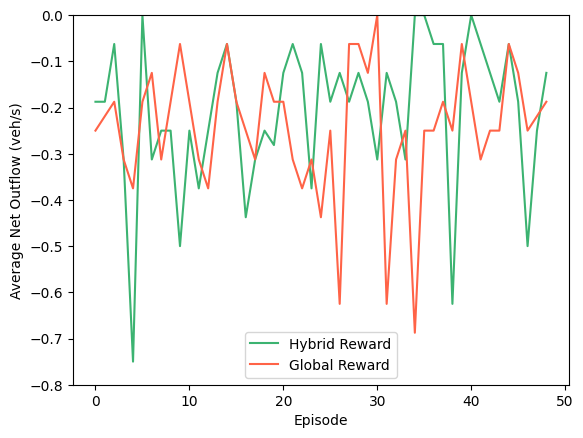
\includegraphics[width=\linewidth]{figs/global_vs_hybrid.png}
            \caption{This project.}
            \label{fig-sub:global-hybrid-my}
        \end{subfigure}
        \begin{subfigure}[b]{0.45\linewidth}
            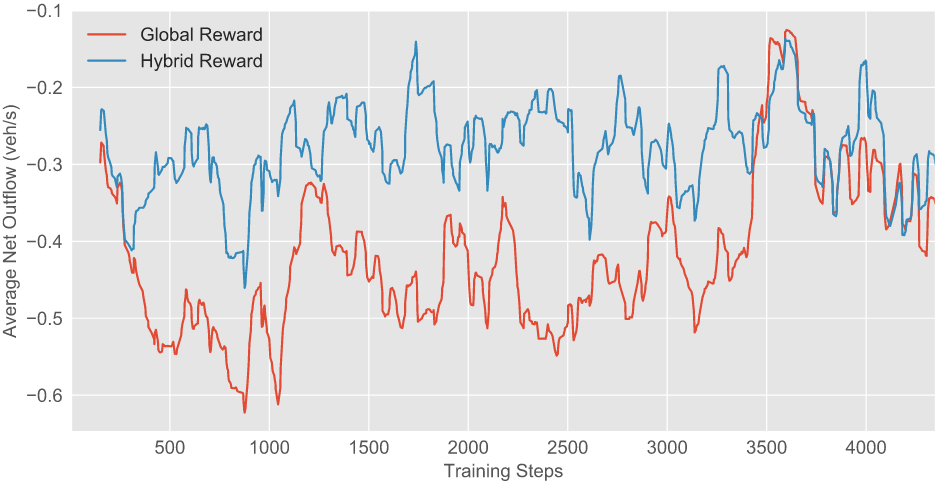
\includegraphics[width=\linewidth]{figs/global_vs_hybrid_reference.png}
            \caption{Original work.}
            \label{fig-sub:global-hybrid-orig}
        \end{subfigure}
        \caption{
            Median training reward per episode of models from this project and original work.
            While not the same, they both show values on similar scale,
            with both hybrid and global reward versions having between $-0.1$ and $-0.3$ final reward.
            The first episode reward is omitted for scaling purposes.
        }
        \label{fig:global-hybrid-rewards}
    \end{figure}
    As~\cite{sumo} claimed hybrid reward lead to more stable behavior during training, which can be see on Fig.~\ref{fig-sub:global-hybrid-orig}.
    However, I was not able to reproduce such a behavior.
    Overall, both of my models were more volatile, which can be due to difference in clipping parameter schedule.
    Another possible reason is changing routes of vehicles every episode which may lead to less stable behavior inter-episodes.

    The reward ranges are similar between the two trainings showing that while reproducing relative performance relations was not achievable,
    the overall structure of the model is clear enough to train similarly performing agent.

    \subsection{Traffic Lights as a feature}
    \begin{figure}[h]
        \centering
        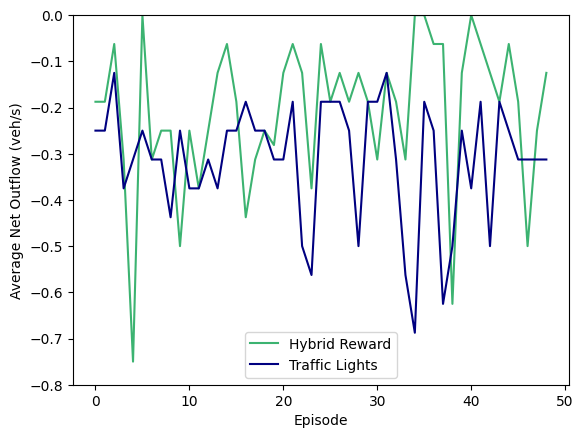
\includegraphics[width=0.5\linewidth]{figs/traffic_light_result.png}
        \caption{
            Median training reward per episode of models with and without traffic lights.
            The first episode reward is omitted for scaling purposes.
        }
        \label{fig:traffic-light-result}
    \end{figure}
    As discussed in Section~\ref{sec-sub:add-feats} addition of traffic lights seems to be a reasonable decision considering that it is a part of state space directly affected by actions.
    However, as shown on Fig.~\ref{fig:traffic-light-result} there is no significant difference in performance between agents using and not using this feature.

    The feature counting number of halted vehicles might be a good proxy for which lights are currently turned on and off,
    causing the two to be highly correlated. This could lead to no differences in adding such a feature.

    The one perhaps desirable feature of adding traffic lights state as a feature is seemingly more stable behavior across episodes.
    As routes change every episode for every agent, the variance in results is to be expected.
    However, with different route patterns the correlation between halted vehicles and traffic light state might differ, in which case having both of the features stabilizes training.
    This would reduced inter-episode variance as seen on a graph.
    However, it can also be due to randomness, and would have to be repeated over many runs to make substantial claims.

    \section{Conclusion and Future Work}
    Overall, I was able to reproduce majority of the results from the original work~\cite{sumo}.
    The main point I failed to reproduce was the relation between hybrid and global reward, which can be due to differences in training processes.

    As mentioned in Section~\ref{sec:intro} the main advantage of this approach is the efficient scaling of the state space with the number of traffic light.
    I would like to further test it on variety of real-life environments.
    In particular the 500m distance between each pair of intersections seems rather large for most city centers,
    and training a model on a denser, busier and overall more challenging environment might give it more room for improvement.

    \bibliography{balbok}
    \bibliographystyle{ieeetr}
\end{document}
